\documentclass[aspectratio=169,12pt]{beamer}
% Compile from the repository root: make presentation
% Ten main slides, with a suggested 600-second speaking plan in the notes.
% Backup slides follow the conclusion and are outside that speaking plan.
% Replace the author field with agreed group names before submission.
% To show notes: replace "hide notes" below with "show notes" and recompile.
% The figures and numerical macros are shared with the checked report.
% If main.Rmd changes, refresh report inputs and reconcile slide prose/tables.
\usepackage[T1]{fontenc}
\usepackage[utf8]{inputenc}
\usepackage{lmodern,amsmath,amssymb,booktabs,graphicx,array}
\usefonttheme{professionalfonts}
\definecolor{navy}{HTML}{174A6E}
\definecolor{teal}{HTML}{00857D}
\definecolor{gray}{HTML}{64737C}
\definecolor{ink}{HTML}{243945}
\setbeamercolor{normal text}{fg=ink,bg=white}
\setbeamercolor{structure}{fg=teal}
\setbeamercolor{frametitle}{fg=navy}
\setbeamercolor{title}{fg=navy}
\setbeamercolor{alerted text}{fg=teal}
\setbeamerfont{title}{size=\fontsize{28}{32}\selectfont,series=\bfseries}
\setbeamerfont{frametitle}{size=\fontsize{21}{24}\selectfont,series=\bfseries}
\setbeamersize{text margin left=8mm,text margin right=8mm}
\setbeamertemplate{navigation symbols}{}
\setbeamertemplate{itemize item}{\color{teal}\small\textbullet}
\setbeamertemplate{bibliography item}[text]
\setbeameroption{hide notes}
\pdfstringdefDisableCommands{\def\translate#1{#1}}
\newif\ifbackup
\backupfalse
\setbeamertemplate{footline}{%
  \begin{beamercolorbox}[wd=\paperwidth,ht=4mm,dp=2.5mm,leftskip=8mm,rightskip=8mm]{normal text}
  \color{gray}\scriptsize Geneva temperature trends\hfill
  \ifbackup Backup \insertframenumber\else\insertframenumber/10\fi
  \end{beamercolorbox}}
\newcommand{\degC}{\ensuremath{^{\circ}\mathrm C}}
\newcommand{\source}[1]{\par\vspace{1.5mm}{\fontsize{8}{9.5}\selectfont\color{gray}#1\par}}
\newcommand{\point}[1]{\par\vspace{2mm}{\color{teal}\bfseries #1\par}}
\graphicspath{{report/figures/}}
\newcommand{\Nobs}{226}
\newcommand{\FirstYear}{1753}
\newcommand{\LastYear}{2013}
\newcommand{\NMissing}{35}
\newcommand{\MeanYear}{1866.4071}
\newcommand{\YMean}{9.5034}
\newcommand{\YSd}{0.6958}
\newcommand{\YMin}{7.6483}
\newcommand{\YMax}{11.7300}
\newcommand{\LinearIntercept}{9.4481}
\newcommand{\LinearSlope}{0.0337}
\newcommand{\DWstat}{1.4147}
\newcommand{\DWLower}{1.7549}
\newcommand{\DWUpper}{2.2695}
\newcommand{\DWp}{0.0002}
\newcommand{\BPstat}{0.4173}
\newcommand{\BPp}{0.5183}
\newcommand{\BreakYear}{1851}
\newcommand{\BrokenIntercept}{9.0690}
\newcommand{\PreSlope}{-0.0525}
\newcommand{\DeltaSlope}{0.1412}
\newcommand{\PostSlope}{0.0887}
\newcommand{\BreakStat}{12.2106}
\newcommand{\SigmaHat}{0.6182}
\newcommand{\Reduction}{12.5305}

\title{Temperature trends\texorpdfstring{\\}{ }in Geneva}
\subtitle{Linear trends, structural change and bootstrap inference}
\author{Computational Methods in Econometrics}
\institute{Vrije Universiteit Amsterdam}
\date{2026--2027}

\begin{document}

% MAIN 1: 25 seconds
\begin{frame}[plain]
\vspace{7mm}
{\usebeamerfont{title}\color{navy}Temperature trends\par in Geneva\par}
\vspace{5mm}
{\large Linear trends, structural change\par and bootstrap inference\par}
\vfill
\insertauthor\par
{\small Vrije Universiteit Amsterdam\par Academic year 2026--2027}\par
\vspace{3mm}
{\color{gray}\small Station08\quad \FirstYear--\LastYear\quad \Nobs\ observed years}
\vspace{4mm}
\note{Suggested time: 25 seconds. We ask whether Geneva's record shows a sustained temperature trend, whether one slope describes it adequately, and how dependence changes inference about a possible change in slope. The analysis retains every supplied observation. The talk follows the empirical diagnostics, the bootstrap comparison and the simulation study. The assignment handout motivates this sequence.}
\end{frame}

% MAIN 2: 60 seconds
\begin{frame}{Geneva's record contains a 29-year gap}
\begin{columns}[T,onlytextwidth]
\column{.70\textwidth}
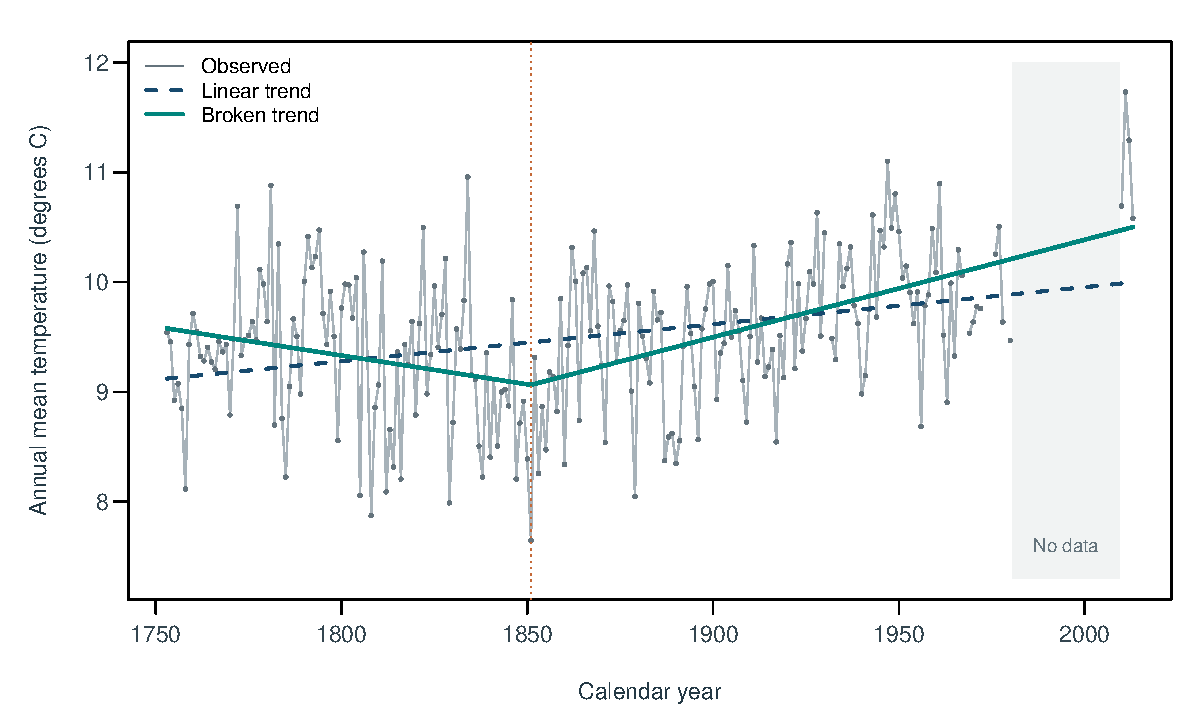
\includegraphics[width=\linewidth]{temperature_fits.pdf}
\column{.27\textwidth}
\vspace{3mm}
\textbf{226 observations}\par
1753--2013\par\vspace{4mm}
\textbf{35 missing years}\par
Five gaps\par\vspace{4mm}
\textbf{1981--2009}\par
Largest gap\par\vspace{4mm}
All observations retained.\par No interpolation.
\end{columns}
\source{Geneva, Switzerland. GHCN-M v4 QCF adjusted series. Annual means require at least ten valid months \cite{menne,stationdata}. Fitted curves across gaps are model-implied.}
\note{Suggested time: 60 seconds. The source metadata identifies Geneva at 46.20 degrees north, 6.15 east and 405 metres elevation. This is the quality-controlled, homogenisation-adjusted series. All 226 temperatures remain, including the final four in 2010--2013. There are no missing cells in the CSV, but 35 absent calendar years. In particular 1980 and 2010 are thirty years apart. The plot shows the two fits that we compare in the talk. Observed lines stop at gaps, while fitted curves express the models. Neither interpolation nor the four final values can reveal the missing trajectory. Source: supplied Station08 metadata and Menne et al. (2018).}
\end{frame}

% MAIN 3: 65 seconds
\begin{frame}{The linear fit leaves residual dependence}
\[
 x_i=\frac{\mathrm{Year}_i-1850}{10},\qquad
 \widehat y_i=\LinearIntercept+\LinearSlope x_i
\]
\vspace{1mm}
\begin{center}\renewcommand{\arraystretch}{1.25}
\begin{tabular}{lrr}
\toprule Diagnostic & Statistic & $p$-value\\\midrule
Durbin--Watson & \DWstat & \DWp\\
Breusch--Pagan & \BPstat & \BPp\\\bottomrule
\end{tabular}\end{center}
\begin{itemize}
\item DW lies below the lower simulated cutoff, \DWLower.
\item BP does not reject against a linear variance trend.
\item Dependence qualifies conventional OLS and BP inference.
\end{itemize}
\source{OLS slope: \degC\ per decade. Primary DW uses observation adjacency and 9,999 iid Gaussian-null simulations. BP uses the nominal $\chi^2_1$ reference \cite{dufour,koenker,bp}.}
\note{Suggested time: 65 seconds. Centring at 1850 makes the intercept fitted temperature in that year. The slope is about 0.034 degrees per decade and is descriptive at this stage. The primary DW statistic follows the assignment's observation-adjacent definition. Both its p-value and the separately calibrated calendar-adjacent sensitivity p-value equal 0.0002. Type-6 cutoffs and strict rejection match the rank rule under the iid Gaussian null. Rejection can reflect residual dependence or an inadequate mean. BP's 0.5183 does not prove constant variance: it targets a linear trend in squared residuals and its usual p-value does not adjust for dependence. Sources: Dufour and Khalaf (2001), Koenker (1981), Breusch and Pagan (1979).}
\end{frame}

% MAIN 4: 60 seconds
\begin{frame}{The best-fitting slope change is in 1851}
\[
 y_i=\alpha+\beta x_i+\delta(x_i-x_k)_++\varepsilon_i
\]
\begin{columns}[T,onlytextwidth]
\column{.64\textwidth}
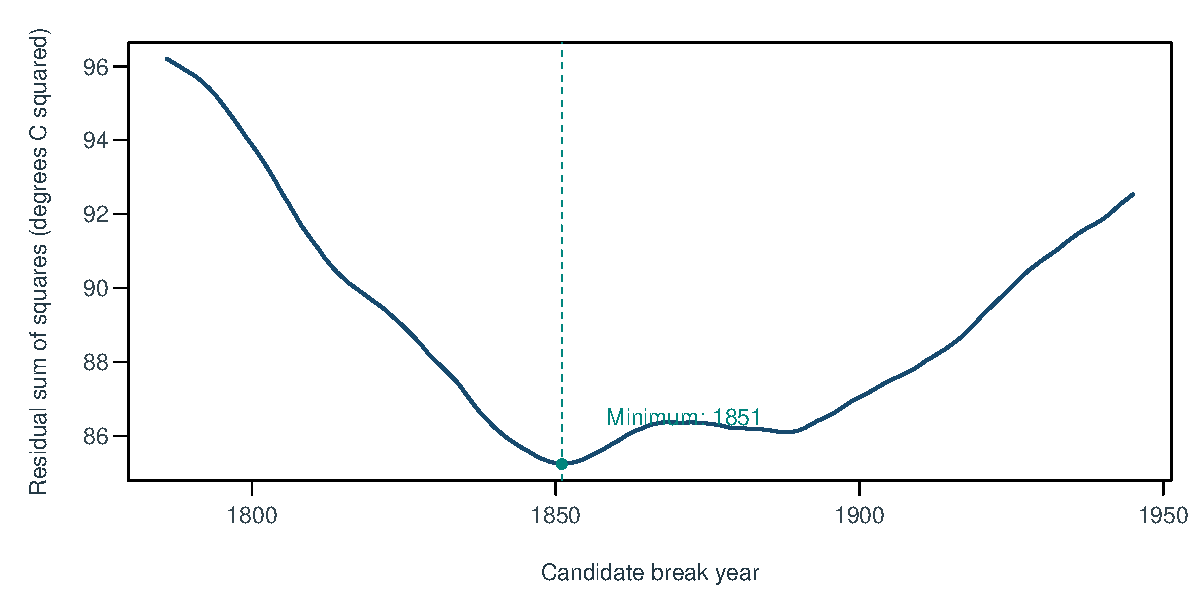
\includegraphics[width=\linewidth]{break_profile.pdf}
\column{.33\textwidth}
15\% trimming by\par observation count\par\vspace{2mm}
Candidates: 1786--1945\par\vspace{2mm}
\textbf{Before:} \PreSlope\par
\textbf{After:} $+\PostSlope$\par
{\small \degC\ per decade}\par\vspace{2mm}
RSS falls by 12.5\%.
\end{columns}
\source{$F_T=RSS_0-\min_k RSS_k=\BreakStat$\,\degC$^2$. Searching the date requires bootstrap calibration \cite{andrews}.}
\note{Suggested time: 60 seconds. The positive-part hinge permits a change in slope while enforcing continuity. The pre-break slope is beta and the later slope is beta plus delta. We trim counts rather than calendar duration because the long gap would otherwise leave very few observations in some candidate regimes. The 159 candidates run from positions 34 through 192. The minimum is at position 99, year 1851. The statistic is the raw RSS reduction specified in the assignment. Under no break the date is unidentified, so searching all these dates invalidates a usual fixed-date test. The selected date is descriptive until we calibrate the search. Source: Andrews (1993).}
\end{frame}

% MAIN 5: 75 seconds
\begin{frame}{Bootstrap error generators}
\begin{center}\small\renewcommand{\arraystretch}{1.3}
\begin{tabular}{lll}
\toprule \textbf{Method} & \textbf{Error draw} & \textbf{Preserves}\\\midrule
IID residual & Resample residuals & Common distribution\\
Independent wild & Residual $\times$ independent sign & Local residual scale\\
Dependent wild & Residual $\times$ correlated weight & Scale and dependence\\\bottomrule
\end{tabular}\end{center}
\[
\operatorname{Corr}(w_i,w_j)=\exp(-|s_i-s_j|/\ell),\qquad \ell=6\text{ years}
\]
\begin{itemize}
\item Generate under the fitted linear null using its residuals.
\item Repeat the full date search in every bootstrap sample.
\end{itemize}
\source{9,999 draws per test. Primary DWB bandwidth: six years. Sensitivities: three and twelve years \cite{wu,liu,shao,friedrich}.}
\note{Suggested time: 75 seconds. IID resampling destroys time dependence and location-specific scale. Independent wild weights preserve each residual's squared scale but remove cross-covariances. DWB uses mean-zero Gaussian weights whose correlation falls with actual calendar distance, including the gaps. At bandwidth six, one-year weight correlation is about 0.85 and a thirty-year gap has correlation about 0.007. These are chosen multiplier correlations rather than estimates of error autocorrelation. All testing samples target the fitted linear null and use its centred, rescaled residuals. Restricted residuals may contain an unmodelled kink, so neither exact size nor monotonic p-values in bandwidth follows automatically. Sources: Wu (1986), Liu (1988), Shao (2010), Friedrich et al. (2020).}
\end{frame}

% MAIN 6: 70 seconds
\begin{frame}{Break evidence depends on the bandwidth}
\begin{center}\small\renewcommand{\arraystretch}{1.3}
\begin{tabular}{lrrl}
\toprule
Procedure & 95\% critical value & $p$-value & At 5\% \\
\midrule
IID residual & 2.643 & 0.0001 & Reject \\
Independent wild & 3.426 & 0.0001 & Reject \\
Dependent wild ($\ell=6$) & 10.592 & 0.0331 & Reject \\
Dependent wild ($\ell=3$) & 8.772 & 0.0206 & Reject \\
Dependent wild ($\ell=12$) & 12.608 & 0.0541 & Do not reject \\
\bottomrule
\end{tabular}

\end{center}
\point{The primary DWB test rejects, but $\ell=12$ does not.}
\vspace{2mm}
Both independent methods reach the simulation floor.\par
Equal minimum p-values cannot resolve smaller tail differences.
\source{RSS gain and critical values in \degC$^2$. Upper-tail p-value: $(1+\text{exceedances})/(B+1)$.}
\note{Suggested time: 70 seconds. The primary DWB p-value is 0.0331, moderate evidence rather than an overwhelming result. At three years it is 0.0206; at twelve it becomes 0.0541. The sequence rises in these runs but need not rise for every dataset. Its sensitivity is larger than the Monte Carlo standard error of roughly 0.0018 at the primary estimate. IID and independent wild each have zero exceedances out of 9,999, giving 0.0001 with the plus-one rule. That is the available resolution, not a zero probability or a confidence bound. Their equality does not establish that heteroskedasticity is unimportant. The simulation will explain why their smaller p-values are less persuasive when dependence is present.}
\end{frame}

% MAIN 7: 60 seconds
\begin{frame}{Both post-break intervals exclude zero}
\begin{columns}[T,onlytextwidth]
\column{.68\textwidth}
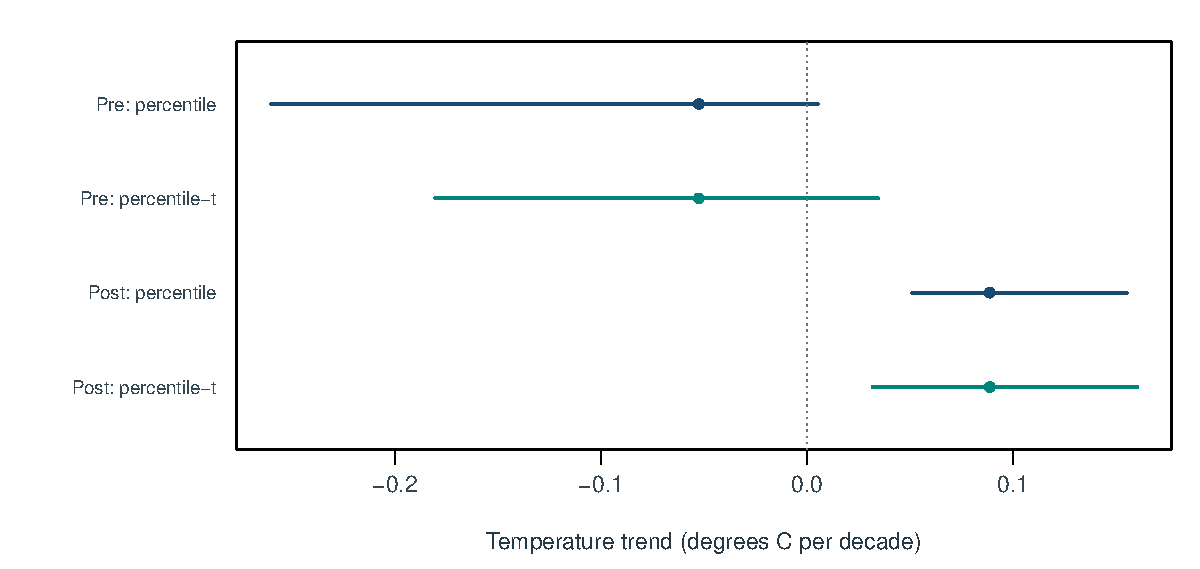
\includegraphics[width=\linewidth]{slope_intervals.pdf}
\column{.29\textwidth}
\vspace{4mm}
\textbf{Pre-break}\par Both intervals include zero.\par\vspace{6mm}
\textbf{Post-break}\par Both intervals exclude zero.
\end{columns}
\vspace{3mm}
Generate under the fitted broken alternative.\par
Reselect the date in all 4,999 draws.
\source{DWB bandwidth six. Percentile-t intervals use calendar-time HAC studentisation \cite{davison,newey}. Interpretation is conditional on the broken-trend specification.}
\note{Suggested time: 60 seconds. Confidence intervals answer a different question from the break test. We now generate around the fitted alternative and use its residuals. Every sample reselects the date, so the estimates incorporate date variation. Percentile intervals use slope quantiles; percentile-t intervals studentise using a newly calculated calendar HAC standard error in every draw. The pre-break point estimate is negative, but both intervals contain zero. Both later intervals are positive, conditional on this fitted specification. They do not independently establish break existence. The local date Jacobian and weak identification make coverage an approximation, and our simulation does not study coverage. Sources: Davison and Hinkley (1997), Newey and West (1987).}
\end{frame}

% MAIN 8: 50 seconds
\begin{frame}{Eight scenarios assess size and power}
\[
 y_t=9.5-0.05x_t+\delta(x_t-x_{113})_++\varepsilon_t,
 \qquad \varepsilon_t=\rho\varepsilon_{t-1}+\sigma_tu_t
\]
\begin{center}\renewcommand{\arraystretch}{1.25}
\begin{tabular}{ll}\toprule
Factor & Values\\\midrule
Slope change $\delta$ & 0 or 0.14\,\degC\ per decade\\
Dependence $\rho$ & 0 or 0.4\\
Innovation scale $\sigma_t$ & Constant or increasing\\\bottomrule
\end{tabular}\end{center}
\begin{itemize}
\item 1,000 datasets per scenario, 499 draws per method.
\item Each dataset has 226 consecutive annual observations.
\item Gaussian innovations and a central break at position 113.
\end{itemize}
\source{8,000 datasets and 24,000 tests. Innovation scale is calibrated to \SigmaHat\,\degC. The experiment does not reproduce the observed missing-year pattern.}
\note{Suggested time: 50 seconds. Delta zero lets us measure false rejection, or size, against a nominal five percent. Delta 0.14 gives power for a reasonably strong kink similar in magnitude to the empirical estimate. We cross dependence and increasing innovation scale, which gives eight scenarios. Increasing scales run from 0.5 to 1.5 and are normalised to the same mean innovation variance. With rho 0.4, marginal error variance increases because innovation variance is held fixed. All three methods test the same simulated datasets. Replication seeds depend on scenario and dataset index, so changing worker scheduling does not change the samples. Simulated x is centred consecutive time in decades.}
\end{frame}

% MAIN 9: 80 seconds
\begin{frame}{Independent methods over-reject under dependence}
\centering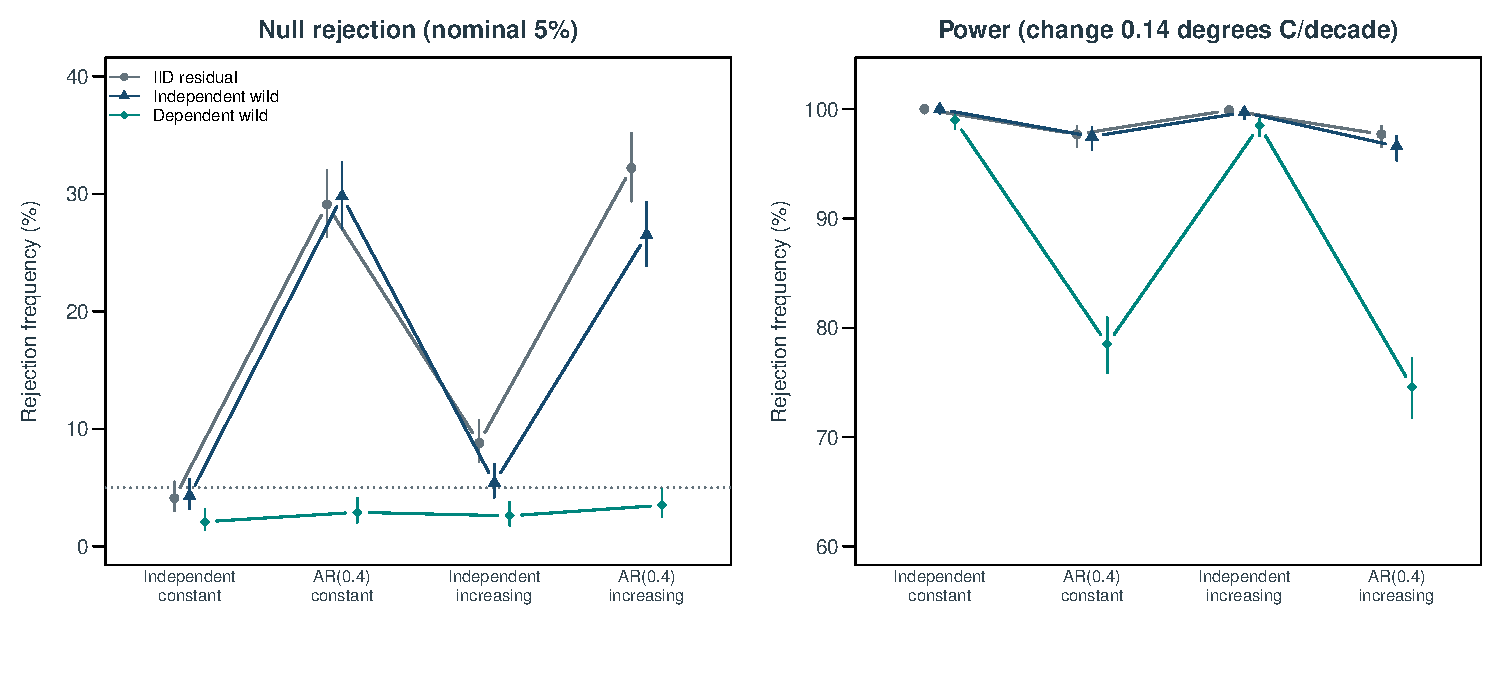
\includegraphics[width=.94\linewidth,height=4.65cm,keepaspectratio]{simulation_results.pdf}
\par\vspace{1mm}\raggedright
\textbf{Under AR(0.4):} independent methods have size 26.5--32.2\%.\par
\textbf{DWB:} size 2.1--3.5\% across scenarios.
\source{95\% Wilson intervals. Panel scales differ. DWB power under dependence: 74.6--78.5\%.}
\note{Suggested time: 80 seconds. The left panel is the key diagnostic of test reliability. Under independence and constant scale, IID and wild sizes are 4.1 and 4.3 percent. Heteroskedasticity alone raises IID size to 8.8 percent while wild stays at 5.4. Serial correlation is more damaging: independent methods reject between 26.5 and 32.2 percent in no-break data. DWB avoids that over-rejection but is conservative in these scenarios, at 2.1 to 3.5 percent. Its power is high under independence but falls to 74.6 to 78.5 percent under AR errors. The independent methods' higher apparent power cannot be treated as better performance when their size is inflated. Wilson intervals measure Monte Carlo sampling uncertainty. These designs do not prove that the empirical DWB p-value is conservative.}
\end{frame}

% MAIN 10: 55 seconds
\begin{frame}{Qualified evidence of a changing trend}
\begin{itemize}
\setlength{\itemsep}{4mm}
\item The fitted later slope is $+\PostSlope$\,\degC\ per decade.\par
Both interval constructions exclude zero.
\item The best-fitting change is near \BreakYear.\par
Its test conclusion is sensitive to the dependence bandwidth.
\item The simulation supports accounting for dependence.\par
DWB remains an approximation with finite-sample limitations.
\end{itemize}
\vspace{3mm}
\point{The missing decades and model assumptions limit stronger claims.}
\source{The later slope averages 1851--2013. It is not a recent-decade rate. A single station and a fitted breakpoint cannot establish a regional transition or physical cause.}
\note{Suggested time: 55 seconds. Return to the research question. The record supports a positive later fitted trend, with intervals that exclude zero under the broken-trend specification. The early slope's uncertainty includes zero. The descriptive curve changes near 1851, but the evidence for a statistically identified break weakens at the longer bandwidth. Dependence matters both in the empirical diagnostics and the simulation. Finish by separating what we estimate from what we do not observe: the 1981--2009 trajectory is unknown, this is one station, and neither a breakpoint nor homogenisation establishes a physical cause. The main talk ends here. Technical backup slides are for questions.}
\end{frame}

\appendix
\backuptrue
\setcounter{framenumber}{0}

\begin{frame}{DW definitions and calibration}
\[
 d_{\mathrm{obs}}=\frac{\sum_{i=2}^n(e_i-e_{i-1})^2}{\sum_i e_i^2},\qquad
 d_{\mathrm{cal}}=\frac{\sum_{i:\,s_{i+1}-s_i=1}(e_{i+1}-e_i)^2}{\sum_i e_i^2}
\]
\begin{center}\small\renewcommand{\arraystretch}{1.2}
\begin{tabular}{lrrrr}\toprule
Definition & Pairs & Statistic & Lower & Upper\\\midrule
Observation adjacency & 225 & 1.4147 & 1.7549 & 2.2695\\
Calendar adjacency & 220 & 1.3865 & 1.7106 & 2.2211\\\bottomrule
\end{tabular}\end{center}
\begin{itemize}
\item Common 9,999 Gaussian draws, each projected off the design.
\item Type-6 cutoffs are order statistics 250 and 9,750.
\item Strict rejection outside cutoffs agrees with $p\leq0.05$.
\end{itemize}
\source{Both two-sided p-values are 0.0002. Exact rank size is conditional on the continuous iid Gaussian null and fixed design \cite{dufour}.}
\note{Use if asked about the gap-adjusted DW statistic. Restricting pairs defines a different statistic, so it needs its own reference distribution. The assignment's observation-adjacent definition remains primary. The p-value doubles the smaller plus-one tail probability and caps at one. A pivotal statistic under the Gaussian null need not have the same distribution under non-Gaussian independent errors. BP can also be calibrated by simulation under a fully specified iid Gaussian null; squared residuals do not make simulation impossible.}
\end{frame}

\begin{frame}{Testing and interval bootstraps target different models}
\begin{columns}[T,onlytextwidth]
\column{.48\textwidth}
\textbf{Break test}\par\vspace{2mm}
Null mean $\widehat y_0$ and residuals $e_0$.\par\vspace{2mm}
Scale residuals by $\sqrt{n/(n-2)}$.\par\vspace{2mm}
Repeat the full search and count $F_T^*\geq F_T$.
\column{.48\textwidth}
\textbf{Slope intervals}\par\vspace{2mm}
Alternative mean $\widehat y_1$ and residuals $e_1$.\par\vspace{2mm}
Scale residuals by $\sqrt{n/(n-3)}$.\par\vspace{2mm}
Reselect the date and recompute slopes and standard errors.
\end{columns}
\vspace{5mm}
\[
 J_i=[1,x_i,(x_i-\tau)_+,-\widehat\delta\,1(x_i>\tau)],\qquad
 K_{ij}=\max\{1-|s_i-s_j|/7,0\}
\]
\source{Studentisation includes the local date direction and uses correction $n/(n-4)$. A rescaled indicator replaces the fourth column for numerical stability when the kink is nonzero. Weak identification can limit coverage.}
\note{The residual scaling and the HAC correction answer different questions. Three linear coefficients determine the alternative residual scale, while the local Jacobian includes the estimated date as a fourth direction. The code rescales that derivative to an indicator. Calendar matching includes only observed pairs at one through six years. Percentile-t intervals reverse the bootstrap t quantiles before subtracting from the observed slope. The source's independent checks reconstruct both interval types from all stored draws. See CODE_GUIDE.md, chunks 30--32.}
\end{frame}

\begin{frame}{The main shape persists in reduced samples}
\begin{center}\small\renewcommand{\arraystretch}{1.4}
\begin{tabular}{lrrrr}\toprule
Sample & $n$ & Break year & Pre slope & Post slope\\\midrule
Full sample & 226 & 1851 & -0.0525 & 0.0887\\
Omit 1851 & 225 & 1853 & -0.0464 & 0.0872\\
End in 1980 & 222 & 1850 & -0.0477 & 0.0776\\\bottomrule
\end{tabular}\end{center}
\begin{itemize}
\item Each reduced sample repeats the trimmed break search.
\item These are descriptive checks without new bootstrap tests.
\item Primary inference retains all 226 observations.
\end{itemize}
\source{Slopes are \degC\ per decade. Alternative-bootstrap date percentiles are 1793 and 1896, with 1.54\% of selections at boundaries. These do not constitute a calibrated break-date confidence set.}
\note{The coldest observation occurs at the estimated full-sample break, making the first sensitivity useful. Removing it shifts the selected year by only two years. Dropping the four post-gap observations lowers the later slope but preserves the fitted direction. These checks do not establish robustness of p-values, since we do not report new inferential calibrations for the reduced samples. Date uncertainty in the alternative bootstrap is wide and explains some asymmetry in the slope intervals.}
\end{frame}

\begin{frame}{Dependence remains after fitting the break}
\begin{columns}[T,onlytextwidth]
\column{.69\textwidth}
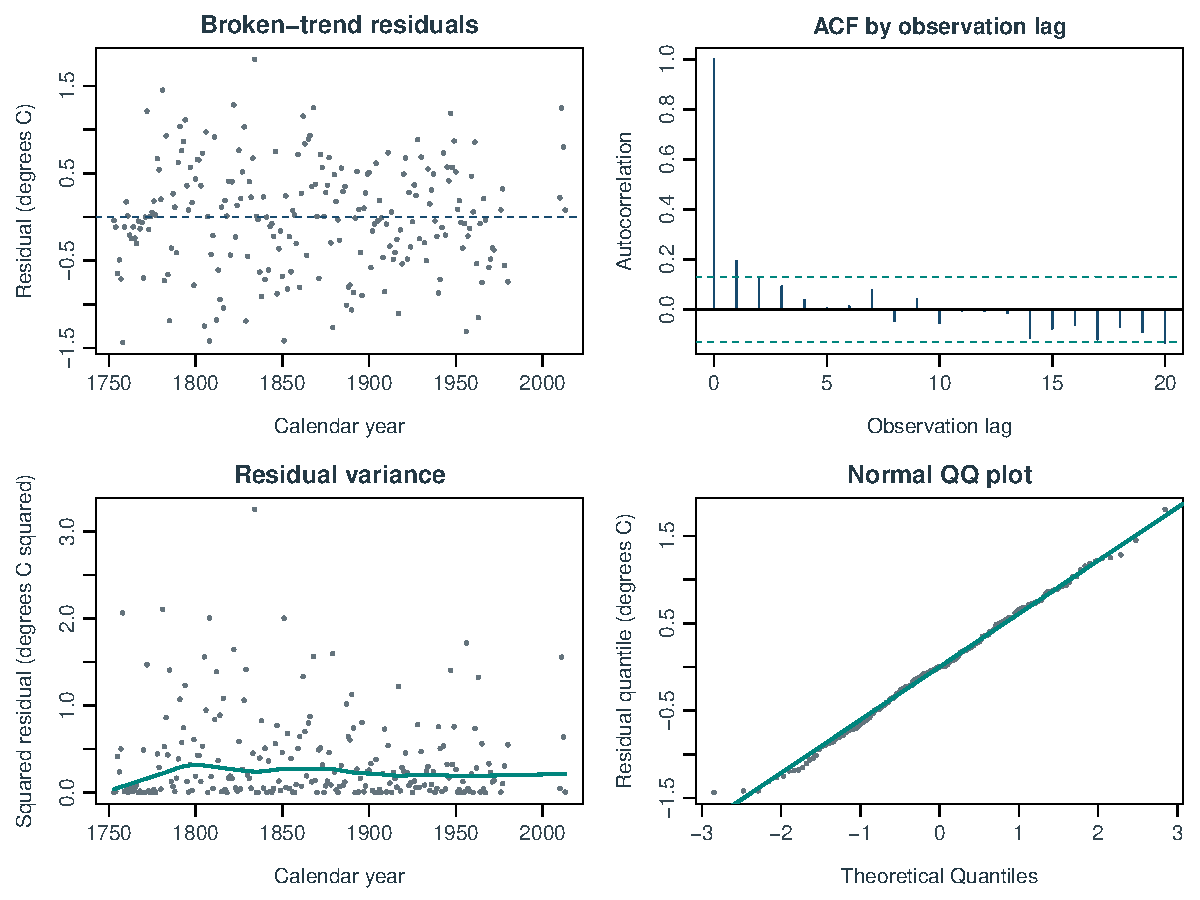
\includegraphics[width=\linewidth,height=5.8cm,keepaspectratio]{diagnostics_broken.pdf}
\column{.28\textwidth}
\vspace{4mm}
ACF(1):\par 0.290 to 0.194\par\vspace{4mm}
DW:\par 1.415 to 1.613\par\vspace{4mm}
RSS reduction:\par 12.53\%\par\vspace{4mm}
Dependence remains.
\end{columns}
\source{Observation lags in the ACF. Selecting a date changes the design, so the linear-model DW critical values do not calibrate a test here.}
\note{The broken mean reduces low-frequency structure, but it does not whiten the residuals. This supports keeping dependence in the interval procedure. The selected model's BP p-value is about 0.209 and remains qualified by the diagnostic's narrow alternative and dependence. In-sample fit measures and a heuristic BIC favour the broken curve, but neither replaces the bootstrap search test.}
\end{frame}

\begin{frame}[allowframebreaks]{References}
\scriptsize
\begin{thebibliography}{99}
\bibitem{handout} Friedrich, M. (2026). \emph{Investigating Temperature Trends: From Linear Trends to Structural Change}. Computational Methods in Econometrics assignment handout, Vrije Universiteit Amsterdam.
\bibitem{menne} Menne, M. J., et al. (2018). The Global Historical Climatology Network Monthly Temperature Dataset, Version 4. \emph{Journal of Climate}, 31, 9835--9854. \href{https://doi.org/10.1175/JCLI-D-18-0094.1}{doi:10.1175/JCLI-D-18-0094.1}.
\bibitem{stationdata} NOAA NCEI. GHCN-M v4, QCF adjusted series. Supplied \texttt{Station08.csv} and \texttt{Station08\_metadata.pdf}. \href{https://doi.org/10.7289/V5XW4GTH}{doi:10.7289/V5XW4GTH}.
\bibitem{andrews} Andrews, D. W. K. (1993). Tests for parameter instability and structural change with unknown change point. \emph{Econometrica}, 61, 821--856. \href{https://doi.org/10.2307/2951764}{doi:10.2307/2951764}.
\bibitem{wu} Wu, C. F. J. (1986). Jackknife, bootstrap and other resampling methods in regression analysis. \emph{Annals of Statistics}, 14, 1261--1295. \href{https://doi.org/10.1214/aos/1176350142}{doi:10.1214/aos/1176350142}.
\bibitem{liu} Liu, R. Y. (1988). Bootstrap procedures under some non-i.i.d. models. \emph{Annals of Statistics}, 16, 1696--1708. \href{https://doi.org/10.1214/aos/1176351062}{doi:10.1214/aos/1176351062}.
\bibitem{shao} Shao, X. (2010). The dependent wild bootstrap. \emph{JASA}, 105, 218--235. \href{https://doi.org/10.1198/jasa.2009.tm08744}{doi:10.1198/jasa.2009.tm08744}.
\bibitem{friedrich} Friedrich, M., Smeekes, S., and Urbain, J.-P. (2020). Autoregressive wild bootstrap inference for nonparametric trends. \emph{Journal of Econometrics}, 214, 81--109. \href{https://doi.org/10.1016/j.jeconom.2019.05.006}{doi:10.1016/j.jeconom.2019.05.006}.
\bibitem{davison} Davison, A. C., and Hinkley, D. V. (1997). \emph{Bootstrap Methods and Their Application}. Cambridge University Press, Chapter 5. \href{https://doi.org/10.1017/CBO9780511802843}{doi:10.1017/CBO9780511802843}.
\bibitem{newey} Newey, W. K., and West, K. D. (1987). A simple, positive semi-definite, heteroskedasticity and autocorrelation consistent covariance matrix. \emph{Econometrica}, 55, 703--708. \href{https://doi.org/10.2307/1913610}{doi:10.2307/1913610}.
\bibitem{koenker} Koenker, R. (1981). A note on studentizing a test for heteroscedasticity. \emph{Journal of Econometrics}, 17, 107--112. \href{https://doi.org/10.1016/0304-4076(81)90062-2}{doi:10.1016/0304-4076(81)90062-2}.
\bibitem{bp} Breusch, T. S., and Pagan, A. R. (1979). A simple test for heteroscedasticity and random coefficient variation. \emph{Econometrica}, 47, 1287--1294. \href{https://doi.org/10.2307/1911963}{doi:10.2307/1911963}.
\bibitem{dufour} Dufour, J.-M., and Khalaf, L. (2001). Monte Carlo test methods in econometrics. In \emph{A Companion to Theoretical Econometrics}, Chapter 23, 494--519. \href{https://jeanmariedufour.github.io/Dufour_Khalaf_1998_MCTCompanion_W.pdf}{Author manuscript}.
\end{thebibliography}
\end{frame}

\end{document}
